\documentclass{scrreprt}
% input encoding
\usepackage[utf8]{inputenc}
\usepackage[T1]{fontenc}
\usepackage{biblatex}
\addbibresource{quellen.bib}
% new german spelling
\usepackage[ngerman]{babel}
% choose font
\usepackage{mathpazo}
% color and images
\usepackage[dvipsnames]{xcolor}%\usepackage{color}
\usepackage{graphicx}
\usepackage{svg}
% quotes
\usepackage[german=guillemets]{csquotes}
% math
\usepackage{amsmath}
\usepackage{amssymb}
% Plotter Funktionen
\usepackage{tikz}
\usetikzlibrary{intersections}
%Inhaltsverzeichnis und Nummerrierung nach standard
\renewcommand{\thesection}{\arabic{chapter}.\arabic{section}}
\setlength{\parindent}{0pt}
%Bilder
\usepackage[section]{placeins}%begrenzt gleiten bilder auf section
% Bessere Unterstützung für PDF-Features
\usepackage[breaklinks=true,hidelinks,hyperfootnotes=false]{hyperref}
\usepackage{cleveref}
\renewcommand{\namecref}{Abschnitt}
%pdf Seiten einbinden
\usepackage{pdfpages}
%Inhaltsverzeichnis und Nummerrierung nach standard
\renewcommand{\thesection}{\arabic{chapter}.\arabic{section}}
\setlength{\parindent}{0pt}
%linenumbers
\usepackage{lineno, blindtext}
\renewcommand{\namecref}{Abschnitt}
% Snippet Highlighting
\usepackage{listings}
\lstset{escapeinside={<@}{@>}}
\renewcommand{\lstlistingname}{Quelltext}% Listing -> Quelltext
\renewcommand{\lstlistlistingname}{List of \lstlistingname s}% List of Listings -> List of Algorithms      %#718a62
\usepackage{upquote}
%Define the listing package
%caption
\lstset{literate=%
	{Ö}{{\"O}}1
	{Ä}{{\"A}}1
	{Ü}{{\"U}}1
	{ß}{{\ss}}1
	{ü}{{\"u}}1
	{ä}{{\"a}}1
	{ö}{{\"o}}1,
	captionpos=b
}

\lstdefinestyle{basiclst} {%
	% General design
	%  backgroundcolor=\color{editorGray},
	basicstyle={\footnotesize\ttfamily},   
	frame=b,
	% line-numbers
	xleftmargin={0.75cm},
	numbers=left,
	stepnumber=1,
	firstnumber=1,
	numberfirstline=true,	
	% Code design
	alsodigit={.:;},	
	tabsize=2,
	showtabs=false,
	showspaces=false,
	showstringspaces=false,
	extendedchars=true,
	breaklines=true,
	% German umlauts
	literate=%
	{Ö}{{\"O}}1
	{Ä}{{\"A}}1
	{Ü}{{\"U}}1
	{ß}{{\ss}}1
	{ü}{{\"u}}1
	{ä}{{\"a}}1
	{ö}{{\"o}}1
}
%dracula color theme
\usepackage{draculatheme}
%highlighter comand
\newcommand{\code}[1]{\texttt{#1}} % inline code setting
\newcommand*{\quelle}{%
  \footnotesize Quelle:
}
\usepackage{mathtools}
\usepackage{ marvosym }
\usepackage[backend=biber, %% Hilfsprogramm "biber" (statt "biblatex" oder "bibtex")
style=authoryear, %% Zitierstil (siehe Dokumentation)
natbib=true, %% Bereitstellen von natbib-kompatiblen Zitierkommandos
hyperref=true, %% hyperref-Paket verwenden, um Links zu erstellen
]{biblatex}

%Zeilenabstand 
\usepackage[singlespacing]{setspace} % doublespacing, onehalfspacing, mehr infos unter: https://www.namsu.de/Extra/pakete/Setspace.html

\makeatother

\title{Dokument}
\author{xi72yow}
\date{März 2022}

\begin{document}

%\includepdf[pages={1}]{data/docs/Deckblatt.pdf} % site of the pdf

\begin{titlepage}
	\maketitle
\end{titlepage}

\tableofcontents
\newpage

\chapter{Lorem Ipsum}


\section{Lorem X\cite{RPOI2003}}
Culpa wie in Abbildung \ref{fig:GidSys} oder in Snippet\footnote{Ich weiß viele	sehen das ganz anders und zitieren auch in oder mit Fußnoten.} \ref{lst:docRenderMap} fugiat laboris mollit sint sunt. Laborum Lorem Lorem deserunt velit sint minim laborum consequat sunt elit laboris. Reprehenderit et ad ex ut consectetur et id adipisicing nulla ex cillum. Amet magna ex exercitation adipisicing eu amet irure anim. Quis laborum veniam elit sint aute. Velit proident aliquip nostrud ullamco tempor dolore cupidatat velit nulla qui exercitation. \\

Deserunt est sint esse ex cillum duis deserunt ea officia veniam Lorem elit nulla. Pariatur laborum ipsum quis Lorem consequat aute ea mollit. Laborum fugiat veniam duis minim dolore adipisicing dolor in labore.

\begin{description}
	\item[Loremer:] Officia fugiat esse minim incididunt excepteur ex voluptate eiusmod velit. Reprehenderit et culpa commodo laboris est est enim enim. Commodo eu magna elit mollit consequat deserunt est.
	\item[Spice:] Excepteur amet Lorem deserunt est ullamco ut irure commodo ipsum aute. Consequat sunt nisi officia eu labore cupidatat pariatur in mollit consequat Lorem dolor exercitation. Esse incididunt laboris quis quis sint. Magna velit ullamco deserunt voluptate et aliquip officia mollit et ex deserunt dolore. Aliquip occaecat cillum sit excepteur sint exercitation nisi cillum Lorem officia. Nulla ipsum consectetur eu tempor minim dolore ex aliquip adipisicing dolore. Quis fugiat et laborum cillum Lorem aliquip pariatur.
	      \begin{figure}[h]
		      \centering
		      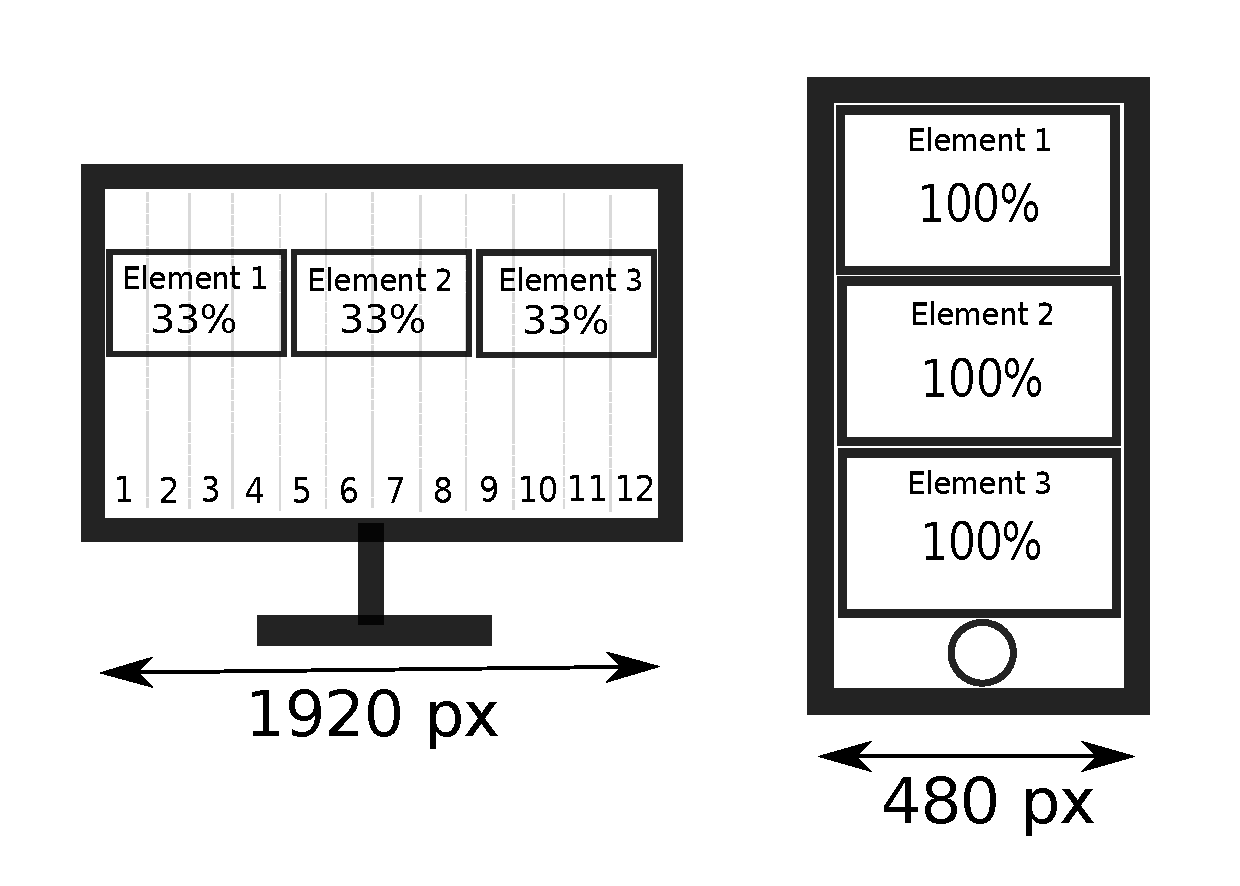
\includegraphics[width=0.8\textwidth,clip]{data/figures/gridSystem.pdf}
		      \caption{Twelve Column Grid auf einem großen und kleinen Bildschirm}
		      \label{fig:GidSys}
	      \end{figure}
\end{description}

\section{Lorem Y}
Laboris laboris anim deserunt laboris laborum est.

\subsection{Lorem ipsum}
Culpa labore cupidatat nostrud ullamco nisi ea. Quis sint nostrud pariatur exercitation excepteur ea est dolor ullamco. Sit magna deserunt pariatur dolore dolore occaecat aliquip adipisicing aliqua. Mollit nisi ad voluptate mollit quis esse duis excepteur amet aute deserunt sit. Duis aliquip labore sit quis irure cillum do. Dolore do consequat ut est exercitation dolore nostrud est. Anim irure pariatur est esse tempor ad labore qui. \\

Consequat labore laborum fugiat velit occaecat commodo velit excepteur. Ex cillum laboris aliqua reprehenderit deserunt. In ipsum quis velit pariatur Lorem sit officia aute ea. Sint in exercitation proident ea do. Do aliqua veniam minim est non reprehenderit minim eiusmod laboris excepteur. Laboris in anim occaecat nostrud esse ex sit id eu magna. Excepteur ut velit qui qui sit aliquip tempor amet est. Ullamco pariatur dolor amet eu dolor. Do labore do dolor pariatur dolor aliquip reprehenderit fugiat et nulla sunt.

\begin{minipage}{\linewidth}
	\lstinputlisting[style=basiclst,caption={Dokumentation und Defaultparameter der renderMap-Funktion}, label={lst:docRenderMap}]{data/snippets/mapPreviewDoc.js.txt}
\end{minipage}

\setcounter{footnote}{9}
%....
Wenn mehr als 9 Fußnoten gesetzt werden und als Zähler\footnote{Zählart
	mag keine Korrektur.} Fußnotensymbole verwendet werden gibt es wo die
Verwendung von alphalph eine Fehlermeldung. Jetzt aber nicht mehr.
%...

%% Quellen:
\printbibliography
%Abbildungverzeichnis
\listoffigures

%\includepdf[pages={1}]{data/docs/lorem.pdf} % site of the pdf
%\includepdf[pages=-]{data/docs/lorem.pdf} % whole document


\end{document}